%%\documentclass[a4paper,12pt,oneside]{llncs}
\documentclass[12pt,letterpaper]{article}
\usepackage[right=2cm,left=3cm,top=2cm,bottom=2cm,headsep=0cm]{geometry}

%%%%%%%%%%%%%%%%%%%%%%%%%%%%%%%%%%%%%%%%%%%%%%%%%%%%%%%%%%%
%% Juego de caracteres usado en el archivo fuente: UTF-8
\usepackage{ucs}
\usepackage[utf8x]{inputenc}

%%%%%%%%%%%%%%%%%%%%%%%%%%%%%%%%%%%%%%%%%%%%%%%%%%%%%%%%%%%
%% Juego de caracteres usado en la salida dvi
%% Otra posibilidad: \usepackage{t1enc}
\usepackage[T1]{fontenc}

%%%%%%%%%%%%%%%%%%%%%%%%%%%%%%%%%%%%%%%%%%%%%%%%%%%%%%%%%%%
%% Ajusta maergenes para a4
%\usepackage{a4wide}

%%%%%%%%%%%%%%%%%%%%%%%%%%%%%%%%%%%%%%%%%%%%%%%%%%%%%%%%%%%
%% Uso fuente postscript times, para que los ps y pdf queden y pequeños...
\usepackage{times}

%%%%%%%%%%%%%%%%%%%%%%%%%%%%%%%%%%%%%%%%%%%%%%%%%%%%%%%%%%%
%% Posibilidad de hipertexto (especialmente en pdf)
%\usepackage{hyperref}
\usepackage[bookmarks = true, colorlinks=true, linkcolor = black, citecolor = black, menucolor = black, urlcolor = black]{hyperref}

%%%%%%%%%%%%%%%%%%%%%%%%%%%%%%%%%%%%%%%%%%%%%%%%%%%%%%%%%%%
%% Graficos 
\usepackage{graphics,graphicx}

%%%%%%%%%%%%%%%%%%%%%%%%%%%%%%%%%%%%%%%%%%%%%%%%%%%%%%%%%%%
%% Ciertos caracteres "raros"...
\usepackage{latexsym}

%%%%%%%%%%%%%%%%%%%%%%%%%%%%%%%%%%%%%%%%%%%%%%%%%%%%%%%%%%%
%% Matematicas aun más fuertes (american math dociety)
\usepackage{amsmath}

%%%%%%%%%%%%%%%%%%%%%%%%%%%%%%%%%%%%%%%%%%%%%%%%%%%%%%%%%%%
\usepackage{multirow} % para las tablas
\usepackage[spanish,es-tabla]{babel}

%%%%%%%%%%%%%%%%%%%%%%%%%%%%%%%%%%%%%%%%%%%%%%%%%%%%%%%%%%%
%% Fuentes matematicas lo mas compatibles posibles con postscript (times)
%% (Esto no funciona para todos los simbolos pero reduce mucho el tamaño del
%% pdf si hay muchas matamaticas....
\usepackage{mathptm}

%%% VARIOS:
%\usepackage{slashbox}
\usepackage{verbatim}
\usepackage{array}
\usepackage{listings}
\usepackage{multirow}

%% MARCA DE AGUA
%% Este package de "draft copy" NO funciona con pdflatex
%%\usepackage{draftcopy}
%% Este package de "draft copy" SI funciona con pdflatex
%%%\usepackage{pdfdraftcopy}
%%%%%%%%%%%%%%%%%%%%%%%%%%%%%%%%%%%%%%%%%%%%%%%%%%%%%%%%%%%
%% Indenteacion en español...
\usepackage[spanish]{babel}
\usepackage{pdfpages}
\usepackage{amssymb}

\usepackage{listings}
% Para escribir código en C
% \begin{lstlisting}[language=C]
% #include <stdio.h>
% int main(int argc, char* argv[]) {
% puts("Hola mundo!");
% }
% \end{lstlisting}


\title{Creación de una infraestructura de red de placas Zybo}
\author{Jesús Rodríguez Heras}

\begin{document}
	
	\maketitle
	\begin{abstract} %Poner esto en todas las prácticas de PCTR
		\begin{center}
			En este documento se desarrolla la creación de la infraestructura de red física de placas Zybo, un ordenador y un switch.
		\end{center}
	\end{abstract}
	\thispagestyle{empty}
	\newpage
	
	\tableofcontents
	\newpage
	
	%%\listoftables
	%%\newpage
	
	%%\listoffigures
	%%\newpage
	
	%%%% REAL WORK BEGINS HERE:
	
	%%Configuracion del paquete listings
	\lstset{language=bash, numbers=left, numberstyle=\tiny, numbersep=10pt, firstnumber=1, stepnumber=1, basicstyle=\small\ttfamily, tabsize=1, extendedchars=true, inputencoding=latin1}


\section{Material necesario}
Para la creación de la infraestructura de red física de placas Zybo contaremos con el siguiente material:
\begin{itemize}
	\item Placas Zybo Zynq-7010.
	\item Un ordenador con sistema operativo Linux (Debian 9 Stretch)\footnote{También es posible usar cualquier otra distribución de Linux.} y Windows 7.
	\item Un switch tp-link modelo TL-SG1024D.
	\item Software Vivado.
\end{itemize}


\subsection{Placas Zybo Zynq-7000}
\begin{figure}[h]
	\centering
	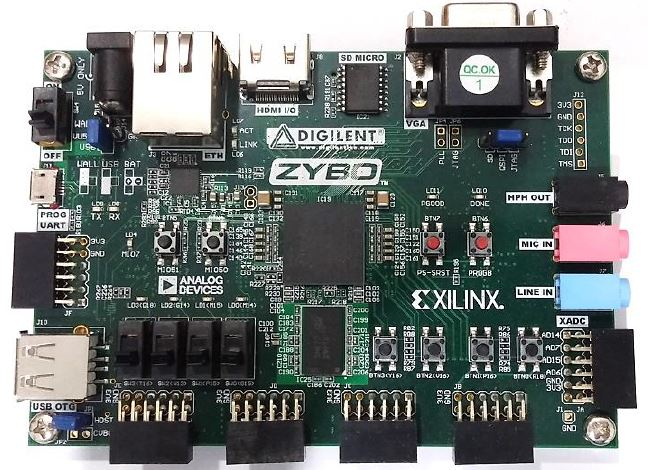
\includegraphics[scale=0.5]{zybo.jpg}
	\caption{Placa Zybo Zynq 7010}
	\label{Placa Zybo}
\end{figure}
Para este proyecto necesitaremos poder programar la FPGA integrada en la placa desde la tarjeta SD de memoria. Para ello se va a preparar una imagen para que el procesador ARM integrado en la placa arranque desde la tarjeta SD y pueda programar la FPGA. El sistema operativo elegido es Xilinux\footnote{Más información en: \url{http://xillybus.com/xillinux}.}.

Las placas Zybo Zynq 7010 tienen tres posibles modos de arranque que podemos seleccionar con el jumper JP5: QSPI, SD, JTAG. En este proyecto, el sistema operativo estará en la tarjeta SD, por lo tanto, tendremos que cambiar el jumper JP5 (situado arriba a la derecha) a la posición ``SD''\footnote{Dicho jumper está identificado con el número 21 en la imagen de la siguiente página.}.
\newpage
\begin{figure}[h]
	\centering
	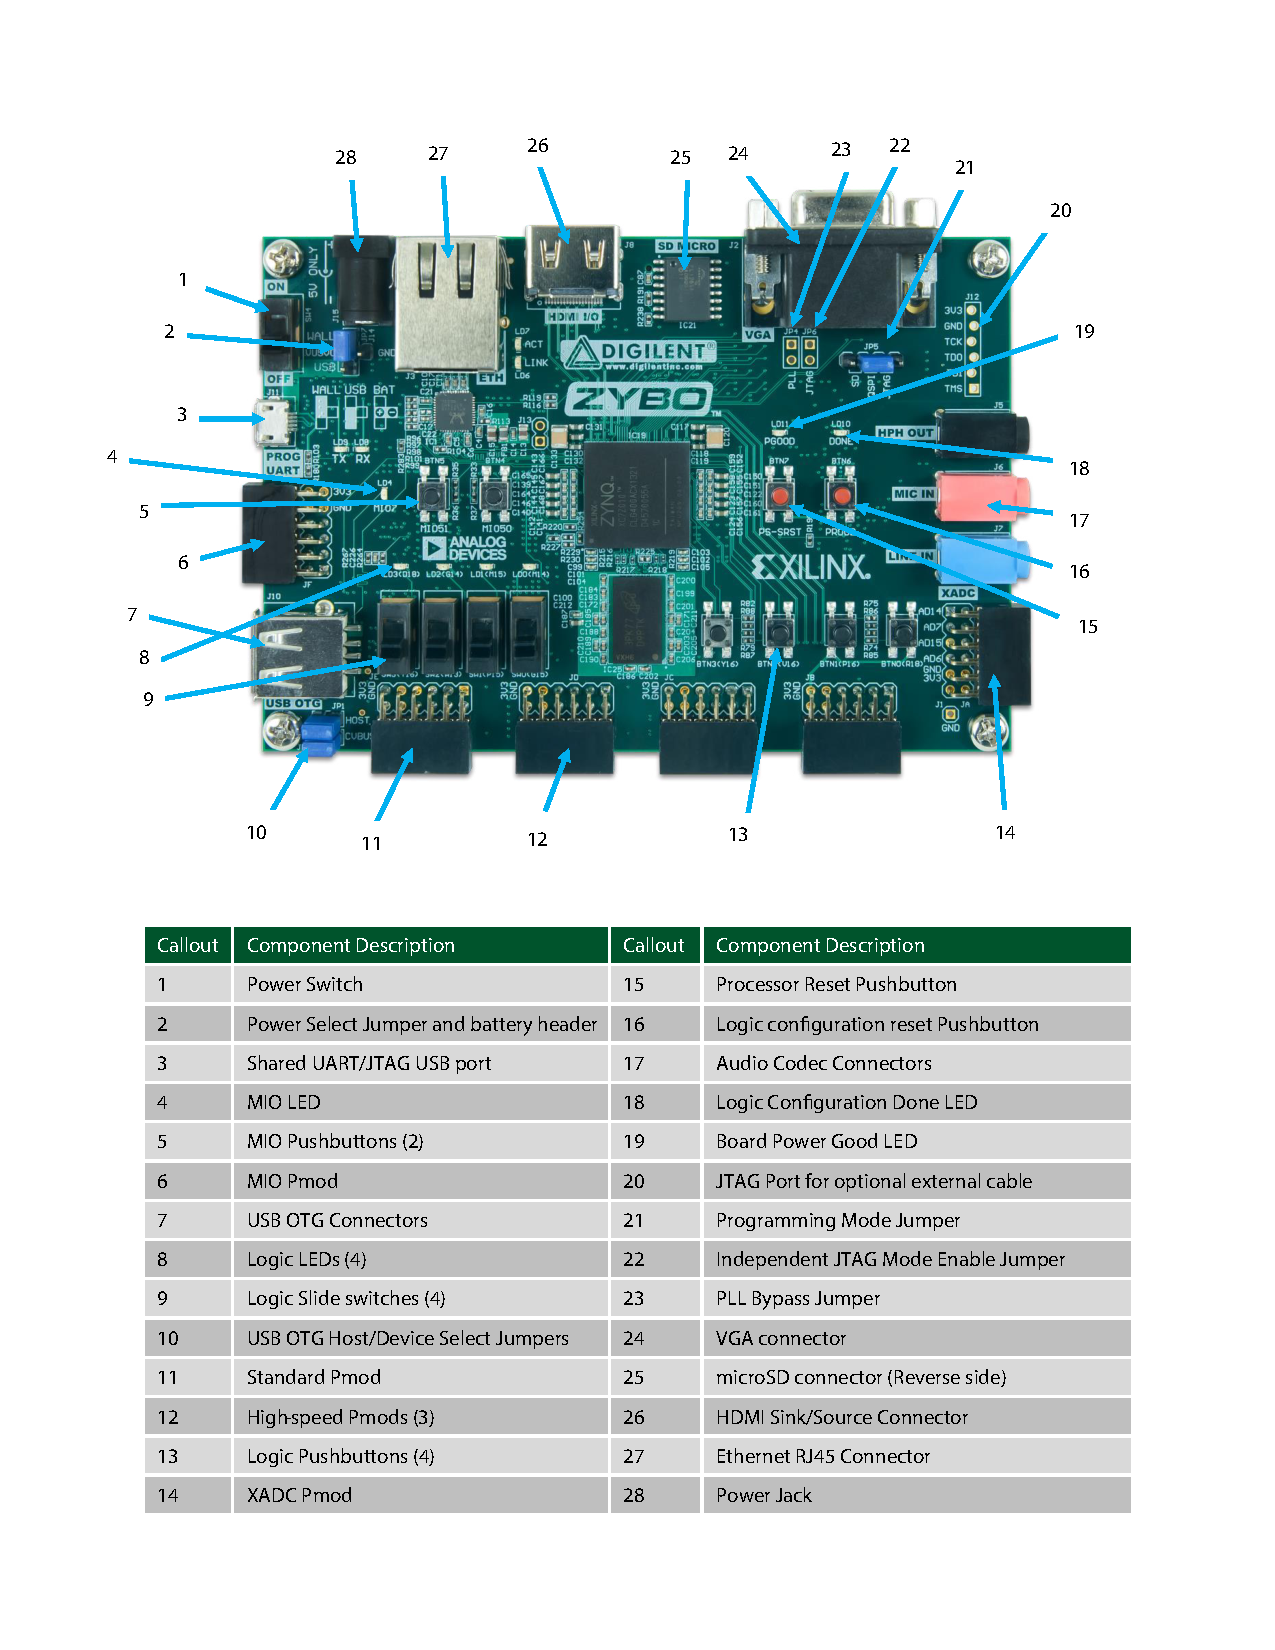
\includegraphics[scale=0.7]{Datasheet.pdf}
	\caption{Diagrama de Zybo Zynq 7010 procedente del manual de referencias}
	\label{Diagrama de Zybo Zynq 7010 procedente del manual de referencias}
\end{figure}
\begin{center}
	\textbf{Fuente:} Manual de referencia oficial de \href{https://reference.digilentinc.com/_media/zybo:zybo_rm.pdf}{\textcolor{blue}{DIGILENT$^{\circledR}$}}.
\end{center}

\newpage
\subsection{Sistemas operativos}
El ordenador usado en el proyecto tendrá dos sistemas operativos.
\begin{itemize}
	\item \textbf{Debian 9 Stretch:} Este sistema operativo tendrá un usuario llamado \texttt{zybo} y su contraseña será \texttt{zybomonitor}. La contraseña para los permisos de super-usuario también será \texttt{zybomonitor}. Este sistema operativo realizará la compilación del sistema operativo Xilinux\footnote{Más información en: \url{http://xillybus.com/xillinux}.} de las tarjetas Zybo a partir de una guía encontrada en GitHub. También realizará la programación del bitstream con el software Vivado y la posterior programación de la FPGA mediante conexión SSH en las placas.
	\item \textbf{Windows 7:} También tendrá la capacidad de programar la FPGA de la tarjeta usando el software Vivado. Será donde, tras los problemas indicados en el tutorial ``Instalación de Linux en SD para Zybo'', tenga lugar la instalación de Xilinux en las tarjetas SD de las placas.
\end{itemize}

\subsection{Software}
\begin{itemize}
	\item \textbf{Vivado:} Versión 2018.2 instalado en los sistemas operativos anteriormente mencionados.
\end{itemize}

\subsection{Switch}
El switch usado en este proyecto es el tp-link TL-SG1024D que cuenta con 24 puertos con tecnología Gigabit y conectores RJ-45. También cuenta con interfaz accesible para su configuración.


\section{Pasos para el montaje de la infraestructura}
\subsection{Asignar direcciones IP}
Para asignarles las direcciones de IP a los dispositivos diferenciamos entre:
\subsubsection{Ordenador}
Debemos identificar la interfaz de red con la que estamos trabajando. Para ello, abrimos un terminal y ejecutamos el siguiente comando como super-usuario\footnote{Comando \texttt{su} y contraseña \texttt{zybomonitor}.}:
\begin{center}
	\texttt{ifconfig}
\end{center}
\newpage
\begin{figure}[h]
	\centering
	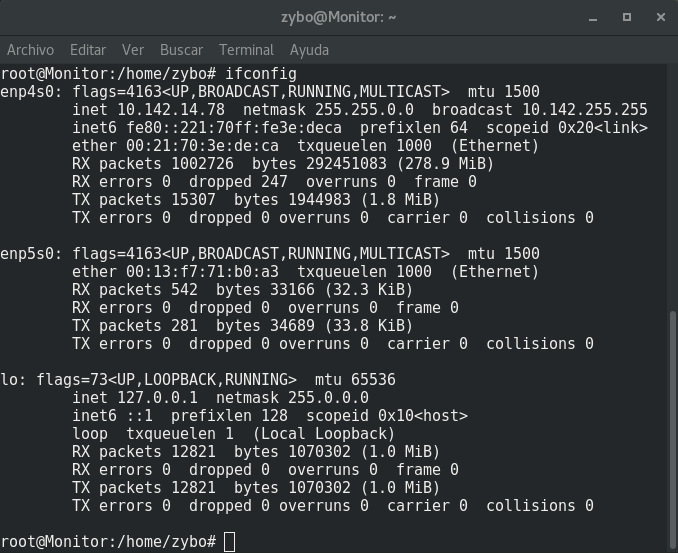
\includegraphics[scale=0.5]{ifconfigPC.png}
	\caption{Interfaces de red del ordenador central}
	\label{Interfaces de red del ordenador central}
\end{figure}

Una vez identificada la interfaz, debemos acceder al fichero\\ \texttt{/etc/network/interfaces.d/INTERFAZ}\footnote{Siendo \texttt{INTERFAZ}, la interfaz que estamos usando. En este ejemplo, \texttt{enp5s0}.} como super-usuario con el siguiente comando:
\begin{center}
	\texttt{gedit /etc/network/interfaces.d/enp5s0}
\end{center}
Y lo modificamos de la siguiente forma:
\begin{lstlisting}
allow-hotplug enp5s0
    iface enp5s0 inet static
    address 192.168.1.10
    netmask 255.255.255.0
    gateway 192.168.1.1
\end{lstlisting}
Configuración del archivo \texttt{/etc/network/interfaces.d/enp5s0} del ordenador central.

\subsubsection{Tarjetas Zybo}
Conectamos la tarjeta mediante USB al ordenador y abrimos un terminal serie en PuTTY\footnote{Puerto ttyUSB1 y velocidad 115200.} e iniciamos sesión en Xilinux\footnote{Usuario: \texttt{zyboX}; contraseña \texttt{zyboX}. Siendo \texttt{X} el identificador de la tarjeta.}.

Debemos identificar la interfaz de red con la que estamos trabajando. Para ello, ejecutamos el siguiente comando como super-usuario\footnote{Comando \texttt{su} y contraseña \texttt{root}.}:
\begin{center}
	\texttt{ifconfig}
\end{center}
\newpage
\begin{figure}[h]
	\centering
	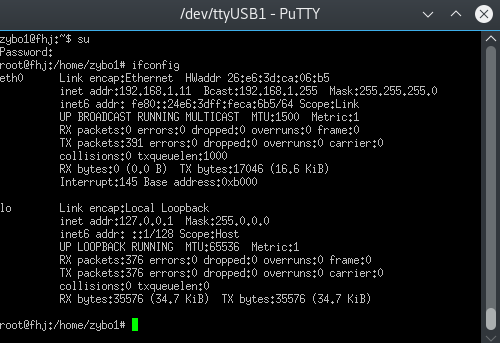
\includegraphics[scale=0.8]{ifconfigZybo.png}
	\caption{Interfaces de red de la tarjeta Zybo}
	\label{Interfaces de red de la tarjeta Zybo}
\end{figure}

Una vez identificada la interfaz, debemos acceder al fichero\\ \texttt{/etc/network/interfaces.d/INTERFAZ}\footnote{Siendo \texttt{INTERFAZ}, la interfaz que estamos usando. En este ejemplo \texttt{eth0}.} como super-usuario con el siguiente comando:
\begin{center}
	\texttt{vi /etc/network/interfaces.d/eth0}
\end{center}
Y lo modificamos de la siguiente forma:
\begin{lstlisting}
allow-hotplug eth0
    iface eth0 inet static
    address 192.168.1.11
    netmask 255.255.255.0
    gateway 192.168.1.1
\end{lstlisting}
Configuración del archivo \texttt{/etc/network/interfaces.c/eth0} para la tarjeta Zybo1.
\newpage
Para establecer la dirección IP del resto de dispositivos, repetiremos el proceso y estableceremos las direcciones IP siguiendo la siguiente tabla:
\begin{table}[h]
	\centering
	\begin{tabular}{|c|c|}
		\hline
		\textbf{Dispositivo} & \textbf{Dirección IP} \\ \hline
		Monitor & 192.168.1.10 \\ \hline
		Zybo1 & 192.168.1.11 \\ \hline
		Zybo2 & 192.168.1.12 \\ \hline
		Zybo3 & 192.168.1.13 \\ \hline
		Zybo4 & 192.168.1.14 \\ \hline
	\end{tabular}
\caption{Direcciones IP de las placas}
\label{Direcciones IP de las placas}
\end{table}

Las tarjetas estarán identificadas como ZyboX (siendo ``X'' el identificador de la placa con la que estamos trabajando) y el ordenador se identificará como ``Monitor''.

Se puede observar que el número identificador de la tarjeta coincide con el último número de la dirección IP $- 10$, de tal forma que si queremos añadir la tarjeta \texttt{Zybo10}, su dirección IP será 192.168.1.20.

\subsection{Conexión al switch de las placas Zybo}
Una vez tengamos los dispositivos identificados tenemos que conectarlos al switch\footnote{Podemos conectar los dispositivos al puerto del switch que queramos debido a que se encargará de ir rellenando su tabla CAM con las direcciones de los dispositivos que tiene conectados.}. No es necesario una configuración previa del switch ni entrar en su interfaz web, ya que no vamos a requerir acciones avanzadas.

Para probar la conectividad entre todos los dispositivos tendremos que ejecutar el test de interconexión de red. Dicho test se encuentra descrito en el documento ``Test de interconexión de red Zybo''.
\end{document}